%==============================================================================
% Section 7: Finite fate of the zero kernel
%==============================================================================
\section{Finite fate of the zero kernel}
\label{sec:finite}

After finding $\dzero$ non-propagating kernel directions at quadratic order, the
natural question is whether these are flat directions (moduli) under finite
deformation, or are blocked by walls at finite amplitude.  This section answers
that question \emph{within the finite Palatini branch / homogeneous
minisuperspace scope}.  \emph{This section is a supporting result and is not part
of Theorem~\ref{thm:rankdefect} (the quadratic theorem).}

\subsection{Classification: exact moduli versus curvature walls}
\label{sec:finite:classification}

For a finite deformation $\beta\mapsto\text{finite value}$ along a kernel
direction, we reconstruct a background-adapted static Palatini branch and verify
the finite expansion (symbolic, up to fourth order) of the reduced energy
density $\Delta(\beta)$.  The result is the following dichotomy:

\begin{itemize}
  \item \textbf{Exact modulus}: $\Delta(\beta)=0$ holds exactly at all orders of
        the expansion (a flat direction persisting under finite deformation).
  \item \textbf{Curvature wall}: $\Delta(\beta)$ develops a curvature-induced
        non-zero term (including a tadpole), and no stationary finite-deformation
        branch exists.
\end{itemize}

\paragraph{Key points at the level of formulas (finite Palatini branch /
homogeneous minisuperspace).}
\begin{itemize}
  \item \textbf{$\Tthree$}: the spatial scalar curvature vanishes identically.
        Hence $\Delta(\beta)\equiv0$ for any kernel direction (exact flat
        homogeneous branch).
  \item \textbf{$\Nilthree$ $\beta_{-}$}: along the tangent vector
        $(\tfrac12,-\tfrac12,0)$ in the Milnor frame, $\Delta(\beta_{-})=0$
        (residual $0$ up to fourth order; exact modulus).  The closed-form branch
        formula is in Appendix~\ref{app:finite:beta}.
  \item \textbf{$\Nilthree$ $\beta_{+}/u$}: along $(-\tfrac12,-\tfrac12,1)$ a
        curvature-induced linear term (tadpole) remains in the reduced energy; a
        curvature wall.
  \item \textbf{$\Solthree$ $\beta_{x}$}: along $(\tfrac13,-\tfrac16,-\tfrac16)$
        a non-zero term remains; no stationary branch (curvature wall).
\end{itemize}

\begin{table}[H]
\centering
\begingroup
\renewcommand{\arraystretch}{1.4}
\begin{tabularx}{\linewidth}{lrrrY}
\toprule
Topology & $\dzero$ & Exact moduli & Curvature wall & Remarks \\
\midrule
$\Tthree$ & 3 & 3 & 0 & exact flat homogeneous moduli \\
$\Nilthree$ & 2 & 1 ($\beta_{-}$) & 1 ($\beta_{+}/u$) &
$\beta_{-}$ exact modulus (residual $0$ to fourth order); $\beta_{+}$ wall with
tadpole \\
$\Solthree$ & 1 & 0 & 1 ($\beta_{x}$) & stationary branch absent \\
$\Sthree$ & 0 & 0 & 0 & $\dzero=0$ endpoint (not applicable) \\
\bottomrule
\end{tabularx}
\endgroup
\caption{Modulus/wall split (finite Palatini branch / homogeneous minisuperspace
scoped).}
\label{tab:modulus}
\end{table}

\begin{figure}[H]
  \centering
  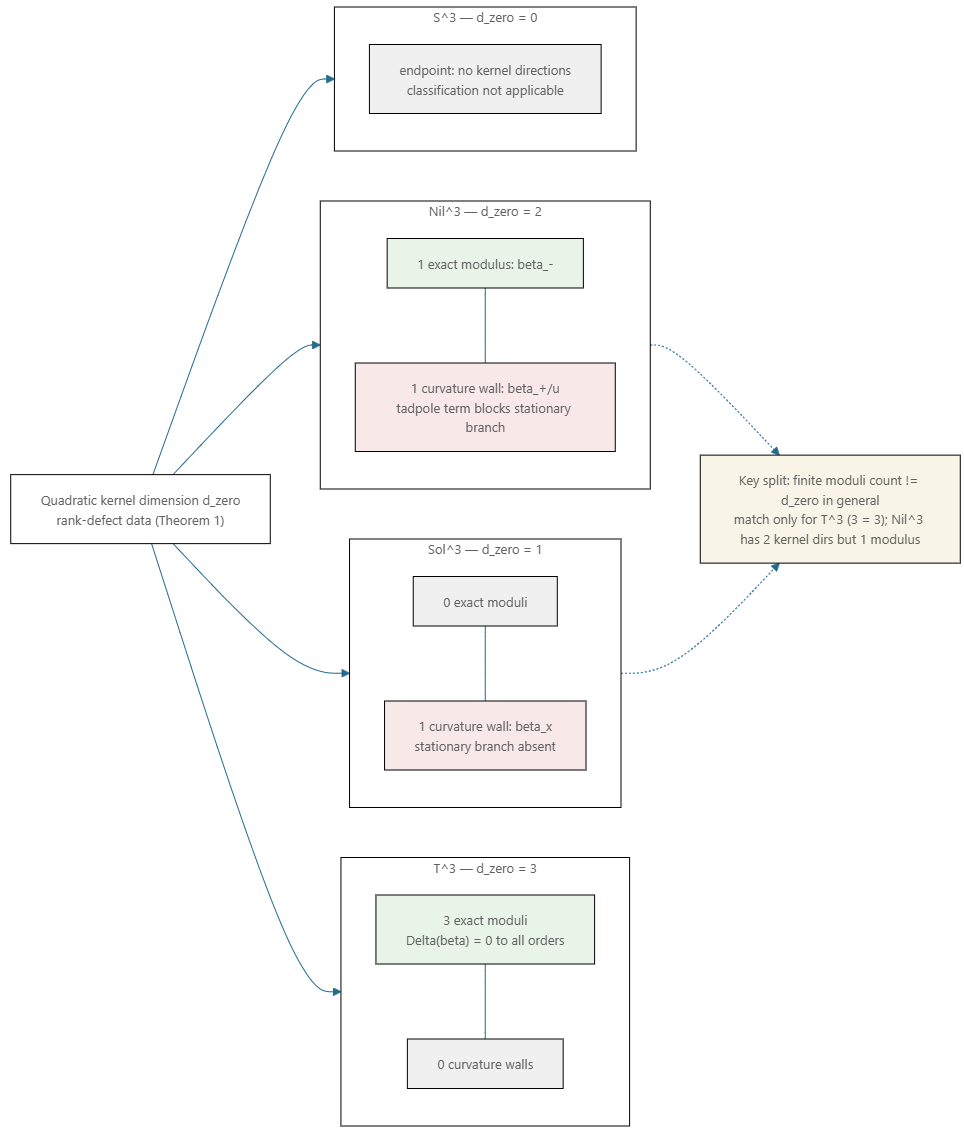
\includegraphics[width=0.95\textwidth]{figures/fig05_Modulus_wall-split.png}
  \caption{Modulus/wall split across the four topologies.  The correspondence
    between the quadratic kernel dimension $\dzero$ and the exact moduli /
    curvature walls on the finite Palatini branch is shown.  $\dzero$ is
    preserved as rank-defect data and does not in general equal the finite moduli
    count (they agree only for $\Tthree$).  \emph{Scope}: the wall checks are
    restricted to the finite Palatini branch / homogeneous minisuperspace; this
    is not a full nonlinear lift theorem.}
  \label{fig:modulus}
\end{figure}

\subsection{Minisuperspace DBR closure}
\label{sec:finite:minisuperspace}

The consistency of this classification was verified with the DBR closure of a
lever-complete homogeneous minisuperspace ansatz including the lapse, the
Hamiltonian constraint, and the DeWitt metric.  The results: (i) the closure
including the Hamiltonian constraint holds; (ii) the DeWitt norm of the
trace-free tangent directions is positive (minisuperspace no-ghost); and (iii)
the configuration degrees of freedom of the homogeneous anisotropy are $2$
(verification data in Appendix~\ref{app:finite}).

\subsection{Mandatory caveats}
\label{sec:finite:caveats}

\begin{itemize}
  \item \textbf{The finite moduli count is not in general equal to $\dzero$.}
        They agree only for $\Tthree$ (3$=$3); for $\Nilthree$ the exact modulus
        is $1$ against $\dzero=2$.  $\dzero$ is preserved as rank-defect data
        (the dimension of the quadratic kernel) and is a different quantity from
        the finite modulus count.
  \item \textbf{The wall checks are established within the finite Palatini
        branch}, and are not a full nonlinear lift theorem or mass theorem.  No
        extension to the time-dependent full DBR dynamics or to the inhomogeneous
        sector is made.
  \item \textbf{The minisuperspace no-ghost is not a full field-theory no-ghost}
        (the analysed scope of the latter is Section~\ref{sec:spectral}).
  \item The energy-density-expansion classification and the stationarity decision
        in the branch reconstruction are distinct checks, presented separately in
        Appendix~\ref{app:finite}.
\end{itemize}

\subsection{Torsion non-contamination (corollary)}
\label{sec:finite:torsion}

The torsion modes (EH/AX/VT/MX) do not change this modulus/wall split.  This is
a corollary of the triviality of the torsion auxiliary shell (not an independent
dynamical check); its precise statement is in Section~\ref{sec:torsion}.
